\chapter{Sätze über kompakte Räume}

\section{Satz von Heine-Borel}
%
Hier ist eine kleine Skizze, die deutlich machen soll, welche Sätze wir als Zutaten für unser Endprodukt, den \glqq Satz von Heine-Borel\grqq, brauchen. \\
%
\\
\input{heineborel_skizze0.pdf_tex}
%

\begin{Satz}\label{satz:beschr}
	Ein kompakter Teilraum \(K\) eines metrischen Raumes \( (X, d) \) ist beschränkt, daher es gilt:
	\[ \exists p \in K, n \in \mathbb{N} : K \subset B_n(p) := \{ x \in X | d(x,p) < n \} \]
\end{Satz}
\beweis{Beweis} 
	Sei \(p \in K\). Das System \( (B_{n}(p) | n \in \mathbb{N}) \) der offenen Kugeln um \(p\) vom Radius \(n \in \mathbb{N}\) 
	überdeckt den gesamten metrischen Raum \(X\), da man für jedes \(x \in X\) ein \(n \in \mathbb{N}\) findet mit \(d(p,x) < n\),
	also mit \(x \in B_{n}(p)\).
	So gilt \(K \subset X = \bigcup_{n \in \mathbb{N}} B_{n}(p)\) und es wird insbesondere auch \(K\) überdeckt. 
	Da \(K\) kompakt ist gibt es ein \(m \in \mathbb{N} : K \subset \bigcup_{i=1}^{m} B_{i}(p) \). Hier ist
	mit eingegangen, dass jede endliche Teilmenge von \(\mathbb{N}\) ein Maximum besitzt.
	Weiterhin gilt \( B_0(p) \subset B_1(p) \subset \dots \subset B_m(p) \) und es folgt \(K \subset B_m(p)\).
\qed

\begin{figure}[ht]
	\centering
	\def\svgwidth{200}
	\input{4_beschraenktheit.pdf_tex}
	\label{fig:beschraenktheit}
	\caption{Illustration zu Satz \ref{satz:beschr}}
\end{figure}

\begin{Satz}\label{satz:intervall}
	Sei \(I = [ a , b ] \subset \mathbb{R}\) ein Intervall mit \(a<b\) und \(a,b \in \mathbb{R}\). Dann 
	ist \(I\) kompakt.
\end{Satz}
\beweis{Beweis} 
	Sei \( (U_{\lambda} | \lambda \in \Lambda) \) offene Überdeckung von \(I\). Zunächst zeigen wir,
	dass ein \(\delta > 0\) existiert mit der Eigenschaft: Für alle \(p \in I\) liegt \(B_{\delta}(p)\)
	in einem \(U_{\lambda}, \lambda \in \Lambda\). Dies kann man auch so ausdrücken: 
	\[ \exists \delta > 0 : \forall p \in I \mbox{ gilt } B_{\delta}(p) \subset U_{\lambda} \mbox { für ein } \lambda \in \Lambda \]
	Wir nehmen an, das Gegenteil sei der Fall:
	\[ \forall \delta > 0 : \exists p(\delta) \in I \mbox{ mit } B_{\delta}(p(\delta)) \not\subset U_{\lambda} \mbox { für alle } \lambda \in \Lambda \]
	Da diese Aussage für alle \(\delta > 0\) gilt, ist es erlaubt \(\delta = \frac{1}{n}\) zu setzen, wobei \(n \in \mathbb{N}\) ist.
	Somit haben wir auf dem Intervall \(I\) eine Folge \(p_{n} := p(\frac{1}{n})\) gefunden mit der Eigenschaft, dass für alle \(\lambda \in \Lambda\)
	gilt: \(B_{\frac{1}{n}}(p_{n}) \not\subset U_{\lambda}\). Nach dem aus der Analysis bekannten Satz von Bolzano-Weiherstraß gibt
	es zu jeder Folge auf dem Intervall \(I\) eine konvergente Teilfolge. Also dürfen wir zu einer konvergenten Teilfolge mit Limes \(p \in I\) übergehen.
  Konvergenz sagt ja gerade aus, dass es zu jeder Umgebung \(U\) von \(p\) ein \(n_0 \in \mathbb{N}\) gibt, 
	ab dem die Folgenglieder in dieser Umgebung verweilen. Dies wiederum heißt, es existiert ein \(B_{\epsilon}(p) \subset U_{\lambda}\) für ein \(\lambda \in \Lambda\)
	(\(p\) muss ja auch in irgendeinem Teil der Überdeckung liegen). Wählt man nun \(n\) so groß, dass \(p_n \in B_{\frac{\epsilon}{2}}(p)\) und \(\frac{1}{n} < \frac{\epsilon}{2}\),
	dann gilt:
	\[ x \in B_{\frac{1}{n}}(p_n) \Rightarrow |x-p| < |p-p_n+p_n-x| < |p-p_n| + |p_n-x| < \frac{\epsilon}{2} + \frac{1}{n} < \epsilon \Rightarrow x \in B_{\epsilon}(p) \]
	Damit ist \(B_{\frac{1}{n}}(p_n) \subset B_{\epsilon}(p) \subset U_{\lambda}\).
	Widerspruch zur Annahme und es gibt für alle \(p \in I\) ein \(\delta > 0\) mit \(B_{\delta}(p) \subset U_{\lambda}, \lambda \in \Lambda\).
	Zerlegt man \(I\) in endlich viele Teilintervalle mit Länge kleiner \(\delta\), so ist jeder dieser Abschnitte ganz in einem \(U_{\lambda}, \lambda \in \Lambda\)
	enthalten. Daher bilden eben jene \(U_{\lambda}\) eine endliche Überdeckung von \(I\).
\qed

\begin{Satz}\label{satz:abgeschlkomp}
		Ist \(X\) kompakt und \(A \subset X \mbox{ abgeschlossen } \Rightarrow A\) kompakt.
\end{Satz}
%
\beweis{Beweis} 
	\\
 	Sei \((F_{\lambda} | \lambda \in \Lambda) \) eine Familie abgeschlossener Teilmengen in \(A\) mit \( \bigcap_{\lambda \in \Lambda } F_{\lambda} = \emptyset \).\\
	Dann ist automatisch auch jedes \(F_{\lambda} \) abgeschlossen in \(X\).\\
	Da \(X\) kompakt ist, besitzt jede Familie \((B_{\omega} | \omega \in \Omega) \) in \(X\) abgeschlossener Mengen mit der Eigenschaft 
	\( \bigcap_{\omega \in \Omega} B_{\omega} = \emptyset\), eine 
	endliche Indexmenge \(\Phi \) für die bereits gilt: \( \bigcap_{\omega \in \Phi} B_{\omega} = \emptyset\).\\
	Also existiert auch eine endliche Indexmenge \( \Gamma \subset \Lambda \) mit \( \bigcap_{\lambda \in \Gamma } F_{\lambda} = \emptyset \), dadurch ist 
	\(A\) auch kompakt.
\qed
		
\begin{Satz}\label{satz:kompabgeschl}
	Ist \(X\) hausdorffsch und \(A \subset X \) kompakt \( \Rightarrow \) \(A\) ist abgeschlossen.
\end{Satz}
%
\beweis{Beweis}
	\\
	Wir wollen zeigen, dass es für jeden Punkt in \(X \backslash A \) eine offene Umgebung in \(X \backslash A \) gibt. Sei daher \(p \notin A \).
	Da \(X\) hausdorffsch ist gilt folgende Aussage:
	\[ \forall a \in A : \exists U_{a} \subset \mathcal{O} \mbox{ mit }  a \in U_{a} \mbox{ und } \exists V_{a}\subset \mathcal{O}, p \in V_{a} 
		 \mbox{ für die gilt } U_{a} \cap V_{a} = \emptyset \] 
	Weiterhin folgt aus der Kompaktheit von \(A\) die Existenz einer endliche Menge \(I \subset A\) mit der Eigenschaft:
	\[ \bigcup_{a \in I} U_{a} = A \]
	Nach Definition eines topologischen Raumes ist der endliche Schnitt \(\bigcap_{a \in I} V_{a}\) offen. Zusätzlich gilt 
	\(p \in \bigcap_{a \in I} V_{a} \subset  X\backslash A \), weil für jedes \(i \in I\) der Schnitt \( ( \bigcap_{a \in I} V_a ) \cap U_i = \emptyset \) ist und 
	somit dieser nicht in \(A\) liegt.
	Also ist eine offene Umgebung von \(p\) in \(X\backslash A\) gefunden und da \(p\) beliebig gewählt war, gilt dies für 
	jeden Punkt \(p \in X\backslash A\). Damit ist \(A\) abgeschlossen. 
\qed
	
\begin{Lemma}[Tubenlemma]\label{satz:tubenlemma}
	Sei \(K \) ein kompakter topologischer Raum,  \(p \in X \) und \( U \subset X \times K \) offen mit \( \{p\} \times K \subset U \). \\
	Dann \( \exists \; V \subset X \), \( V \in \mathcal{O} \) mit \( V \times K \subset U \). \( V \times K \) nennt man \textbf{Tubenumgebung} von 
	\( \{p\} \times K \subset X \times K \).
\end{Lemma} 
%
\beweis{Beweis}
	\\
	\( \forall k \in K \; \exists V_{k}, W_{k}\) offene Mengen mit \( p \in V_{k} \subset X, k \in W_{k} \subset K, (p,k) \in  V_{k} \times W_{k} \subset U\).
	Diese offenen Mengen \(V_{k}, W_{k}\) kann man finden, da laut Vorraussetzung \(U  \subset X \times K \) offen in der Produkttopologie ist.
	Da \(K \) kompakt ist, existiert eine endliche Teilmenge
	\( I \subset K \) mit \( \bigcup_{ k \in I } W_{k} = K \). Wähle \(V := \bigcap_{ k \in I } V_{k} \), dann gilt:
	\[ V \times K \subset \bigcup_{k \in I} (V_{k} \times W_{k}) \subset U \] \qed	\\
%
\begin{figure}[ht]
	\centering
	\def\svgwidth{200}
	\input{tubenlemma.pdf_tex}
	\label{fig:tubenlemma}
	\caption{Illustration zu Lemma \ref{satz:tubenlemma}}
\end{figure}
%
\begin{Satz}
	Ein endliches Produkt hausdorffscher Räume ist wieder hausdorffsch.
\end{Satz}
%
\beweis{Beweis}
	\\
	Wir wollen zunächst zeigen, dass das Produkt zweier hausdorffscher Räume wieder hausdorffsch ist. Dies reicht aus, da man jedes endliche Produkt topologischer Räume
	induktiv auf ein Produkt zweier Räume zurückführen kann. \\
	Seien \(X, Y\) zwei hausdorffsche topologische Räume.\\
	Seien weiter \( (p,q), (x,y) \in X \times Y \mbox{ wobei } (p,q) \ne (x,y) \). \\
	Laut Vorraussetzungen ist \(X\) und \(Y\) jeweils hausdorffsch, also folgt: 
	\begin{align}
		x &\ne p \mbox{ oder }\label{eq:produkt1}\\ 
		y &\ne q\label{eq:produkt2} 
	\end{align}
	Zu \eqref{eq:produkt1} da \(x \ne p \) ist, haben \(x, p \) Umgebungen \(A, B \) mit \( A \in U(x)  \land B \in U(p) \), für die gilt: \(A \cap B = \emptyset \).\\ Daher gibt es die
	zwei Umgebungen \( (A \times Y), (B \times Y) \) mit \( (A \times Y) \cap (B \times Y) = \emptyset \). \\
	Setzt man bei \eqref{eq:produkt2} mit dem gleichen Ansatz an, so folgt leicht, dass \( (X \times Y) \) hausdorffsch ist, da wir gerade gezeigt haben, falls mindestens eine Komponente
	nicht gleich ist, existieren fremde Umgebungen zu zwei nicht gleichen Punktepaaren\( (p,q), (x,y) \), was genau der Definition von hausdorffsch entspricht.
\qed

\begin{Satz}\label{satz:prodkomp}
	Ein endliches Produkt kompakter Räume ist wieder kompakt.
\end{Satz}
	%
	\beweis{Beweis}
	\\
	Wir zeigen wieder zunächst, dass das Produkt zweier kompakter Räume wieder kompakt ist. Hier kann man ebenfalls leicht mittels Induktion jedes endliche Produkt kompakter Räume 
	auf ein Produkt zweier kompakter Räume zurückführen. \\
	Nun seien \(X, Y\) zwei kompakte Räume.\\
	Ist \((U_{\lambda} | \lambda \in \Lambda) \) eine offene Überdeckung in \(X \times Y \). Jede Faser \( \{p\} \times Y, p \in X \) wird von endlich vielen \(U_{\lambda} \) überdeckt,
	da Y kompakt ist. Also gibt es eine Teilmenge \( I \subset \Lambda \) mit \( \{p\} \times Y \subset \bigcup_{ \lambda \in I } \{p\} \times U_{\lambda} \). 
	Nach dem Tubenlemma überdeckt \( \bigcup_{ \lambda \in I } \{p\} \times U_{\lambda} \) noch eine Menge \(\bigcup_{ p \in X } V_{p} \times Y \mbox{ mit } V_{p} \in X \),
	 wobei \( V_{p} \) eine offene Umgebung von \( p \in X \) ist. Da X kompakt ist überdecken, auch hier bereits endlich viele \(V_{p} \mbox{ ganz } X \). 
\qed

\begin{figure}[ht]
	\centering
	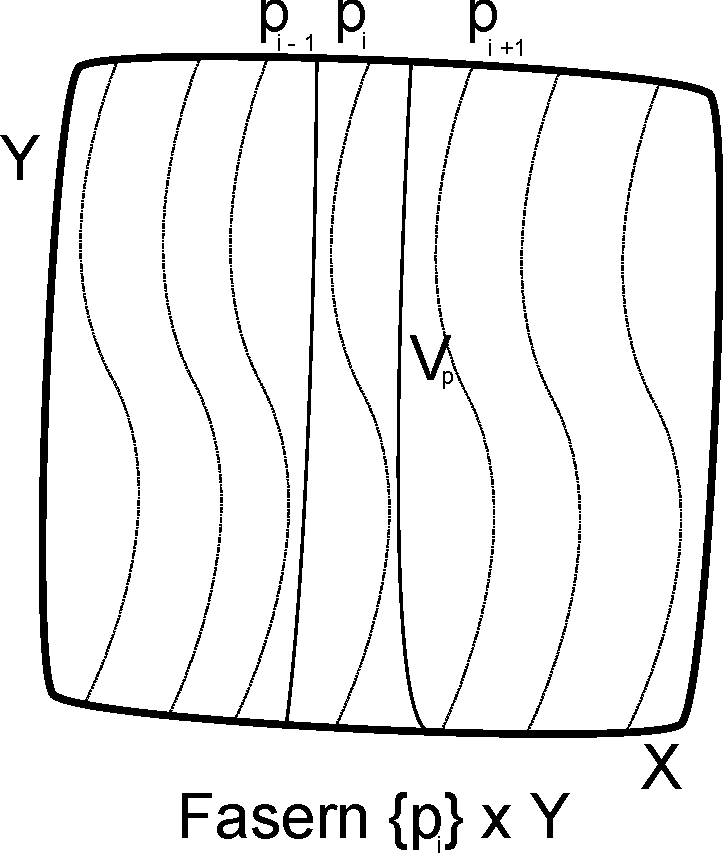
\includegraphics[width=6cm]{produkt_kompakter_raueme.pdf}
	\label{fig:satzprodkomp}
	\caption{Illustration zu Satz \ref{satz:prodkomp}}
\end{figure}
	
\textbf{Bemerkung:} Der Satz von Tychoff zeigt sogar, dass überabzählbare Produkte kompakter Räume wieder kompakt sind. \\
%
\\
Nun können wir endlich zu unserem Hauptziel nämlich dem Satz von Heine-Borel zurück kommen.
%	
\begin{Satz}[Heine-Borel]
	Eine Teilmenge  \( A \subset \mathbb{R}^n \) ist kompakt \(\Leftrightarrow A \) ist abgeschlossen und beschränkt.
\end{Satz}
%
\beweis{Beweis} \\
	Zu \(\Leftarrow \): \\
	Jede abgeschlossene und beschränkte Menge \(A \subset\mathbb{R}^n \), liegt in einem abgeschlossenen n-dimensionalen Würfel
	\( Q_r:= \{ x \in \mathbb{R}^n | \; |x_i| \leq r \quad i=1, \dots, n\} \subset \mathbb{R}^n \). 
	Dies folgt sofort aus der Beschränktheit der Menge \(A\). Der Würfel \(Q_r\) ist als Produkt abgeschlossener und beschränkter Intervalle nach den Sätzen \ref{satz:prodkomp} und \ref{satz:intervall} kompakt.
	Mit Satz \ref{satz:abgeschlkomp} folgt die Kompaktheit der darin enthaltenen abgeschlossenen Mengen.
	\\
	Zu \(\Rightarrow \): \\
	Sei \( K \subset \mathbb{R}^n \) kompakt, dann ist sie laut Satz \ref{satz:kompabgeschl} abgeschlossen und wegen Satz \ref{satz:beschr} ist sie auch beschränkt.
\qed \\
%
\\
\textbf{Bemerkung:} Wichtig ist hierfür aber die Vorraussetzung, dass der topologische Raum, der \(\mathbb{R}^n \) ist. Für metrische Räume ist dieser Satz nicht allgemein gültig. 
Da zum Beispiel mit der trivialen Metrik jede Menge beschränkt ist.
\\
%
Dieser enorm wichtige Satz hat die wunderbare Eigenschaft, dass man in einem sehr oft angewandten Raum, nämlich dem \(\mathbb{R}^n \), 
jetzt relativ leicht entscheiden kann ob eine Teilmenge kompakt ist. 

\section{Weitere}
% 
\begin{Satz}\label{satz:ftk:kompakt}
	Sei \( (X, \mathcal{O}_x) \) ein kompakter Raum und \((Y, \mathcal{O}_y)\) hausdorffscher Raum, sowie \\
	\(f: X \to Y\) stetig.
	Dann ist auch das Bild \( f(X) \) kompakt.
\end{Satz}
%
\beweis{Beweis}
	\\
	Sei \( (U_{\lambda} | \lambda \in \Lambda) \) eine offene Überdeckung von \(f(X)\). Es ist zu zeigen,
	dass eine endliche Teilüberdeckung existiert. 
	\[ f(X) = \bigcup_{\lambda \in \Lambda} U_{\lambda} \Rightarrow X = 
  	 f^{-1}(\bigcup_{\lambda \in \Lambda} U_{\lambda}) = 
		 \bigcup_{\lambda \in \Lambda} f^{-1}(U_{\lambda}) \]
	Da \(f\) stetig ist, sind die Urbilder \( f^{-1}(U_{\lambda}) \) der offenen Mengen \(U_{\lambda}\) wieder offen für 
	alle \(\lambda \in \Lambda\). Somit ist \( ( f^{-1}(U_{\lambda}) | \lambda \in \Lambda ) \) eine offene Überdeckung
	von \(X\). Zu dieser gibt es aufgrund der Kompaktheit von \(X\) ein endliches \( \Gamma \subset \Lambda \), mit 
	der Eigenschaft \( X = \bigcup_{\gamma \in \Gamma} f^{-1}(U_{\gamma}) \). Hieraus folgt:
	\[ f(X) = f(\bigcup_{\gamma \in \Gamma} f^{-1}(U_{\gamma})) = 
  	 \bigcup_{\gamma \in \Gamma} f(f^{-1}(U_{\gamma})) = 
	   \bigcup_{\gamma \in \Gamma} U_{\gamma} \]
\qed

\begin{Satz}
	Sei \((X, \mathcal{O})\) ein kompakter Raum. Dann ist eine stetige Funktion \(f: X \mapsto \mathbb{R}\) 
	beschränkt und nimmt ein Minimum und Maximum an.
\end{Satz}
%
\beweis{Beweis}
	Nach Satz \ref{satz:ftk:kompakt} ist das Bild von \( f(X) \subset \mathbb{R} \) kompakt. Mit Heine-Borel 
	folgt sofort die Beschränkt- und Abgeschlossenheit. Daher enthält \(f(X)\) sein Supremum und Infimum.
\qed
	\begin{Satz}[Satz von Bolzano-Weierstraß]
		Jede Folge in einem kompakten metrischen Raum \(K\) besitzt eine konvergente Teilfolge.
	\end{Satz}
	%
	\beweis{Beweis}\\
		Wir betrachten für beliebige \( p \in K \), die offenen Kugeln \( B_{\frac{1}{n}}(p) \) um \(p \), mit dem Radius \( \frac{1}{n},\; n \in \mathbb{N}\). \\
		Wir nehmen nun an, die Folge besitzt keine konvergente Teilfolge, also in jeder offenen Kugel \( B_{\frac{1}{n}}(p) \) findet man nur endlich viele Folgenglieder. 
		Da K kompakt ist, überdecken endlich viele  \( B_{\frac{1}{n}}(p) \) den ganzen Raum \( K \), daher hätte die Folge insgesamt nur endlich viele Folgenglieder.\\
		Das ist aber ein Widerspruch, da die ganze Folge mit unendlich vielen Folgengliedern im Raum \(K \) wohnt. Also war die Annahme falsch und somit besitzt jede Folge in einem kompakten
		Raum eine konvergente Teilfolge.
	\qed\\
	%
	{\bf Bemerkung:} Die Aussage dieses Satzes ist natürlich äquivalent mit der Aussage, das jede Folge in einem kompakten Raum mindestens einen Häufungspunkt besitzt. 
	%
	

